We presented in the previous chapter the motivations and potential outcomes of conducting a field inference as well as the BORG algorithm. BORG has proven to be very successful 
when applied to galaxy catalogues as well as show great potential regarding weak lensing. Our goal is advance its applications to type Ia supernovae to eventually run it on the 
ZTF data. We will be presenting in this chapter the steps taken in order to achieve the latter. We will start by presenting the ZTF-Uchuu simulations. 
Then the implementation of a an improved supernova-specific likelihood in BORG. 
Then we will present its results on self-consistent simulations. Finally its application to ZTF-like simulations. \\

\section{ZTF-Uchuu mocks}

The ZTF simulations designed to test the impact of ZTF-supernovae peculiar velocities in a cosmological analysis is called DC PV (Data Challenge 
Peculiar Velocity). These are generated within the ZTF collaboration mainly to test methods in inferring $f\sigma_8$. 
The DC PV simulations are done similarly to the DC simulations as 
described in Chapter 4 with the main differences lie in adding structure information to the simulations. For that, the supernovae are simulated with the help of the Uchuu N-body simulation 
(\cite{Ishiyama_2021}), a high fidelity N-body dark matter simulation in a $2^3 \text{Gpc}.h^{-1}$ box with 2.1 trillion particles which can be seen in Figure \ref{fig:uchuu_nbody} \footnote{N-body and hydrodynamical simulations 
are considered the highest fidelity simulations we can get to describe structure formation as they solving the equations of motion for each particle/fluid without any 
approximations or grid mesh}. The full box is then subdivided into 27 subboxes where the supernovae are simulated up to a redshift of $z=0.11$, giving 27 quasi-independent 
realizations of the DC PV. Each supernova must be simulated where a particle is and is assigned the particle's velocity. This allows us to add proper motion to supernovae 
that is driven by structure formation.\\

\begin{figure}[ht]
    \centering
    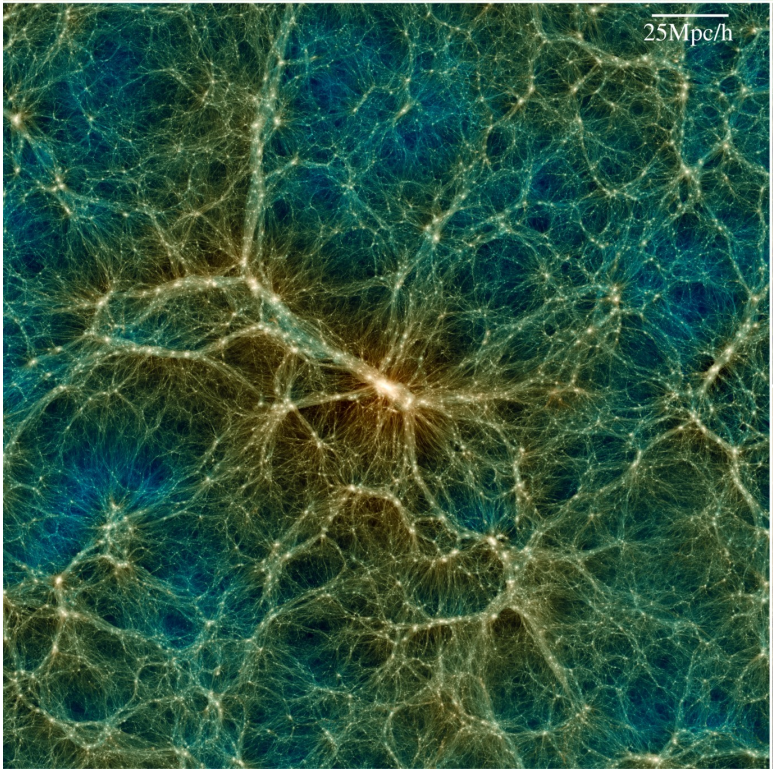
\includegraphics[width=0.7\textwidth]{MainLayout/BORG_chapter/figures/uchuu_nbody.png}
    \caption{Slice taken from the Uchuu simulation covering a box of 250 $\text{Mpc}.h^{-1}$ where each point represents a particle. Taken from \cite{Ishiyama_2021.}}
    \label{fig:uchuu_nbody}
\end{figure}


We opted to simplify a few aspects of the simulations in order to have an initial assessment of how well can a BORG analysis run on ZTF-like supernova. Firstly, we 
have chosen to use only the distance moduli and redshifts of supernovae as inputs in BORG, as if we were doing the analysis after having run the full 
LEMAITRE pipeline. One could assume that in more complicated analyses that the Tripp relation parameters ($\alpha_{\text{Tripp}}$, $\beta_{\text{Tripp}}$) would be sampled in 
BORG. 
This could lead to more acurate results due to the fact that in BORG the 3-dimensional reconstruction of structures in the nearby Universe could accound for non-
Homogenous Malmquist bias. Secondly, we do not impose the ZTF DR2 cosmology quality cuts on photometry nor the ZTF footprint, so all of the supernovae that are 
generated can be used. For a more realistic set of simulations, we would have to account for the geometry of the survey as well as the Milky-Way dust. This means introducing an 
angular mask $M(\text{RA}, \text{Dec})$ in the likelihood's selection function. This method was applied in BORG analyses such as 
\cite{Mcalpine_2025} (Manticore-Local) and \cite{Mcalpine_2026} (Manticore-Deep). Finally, we draw a set of 1000 randomly selected supernovae up to a redshift of $z=0.06$ to 
match the expected number of supernovae in the volume-limited sample from ZTF. We show in Figure \ref{fig:ztf_uchuu} an example of simulated supernovae on top of the Uchuu simulation.\\


\begin{figure}[ht]
    \centering
    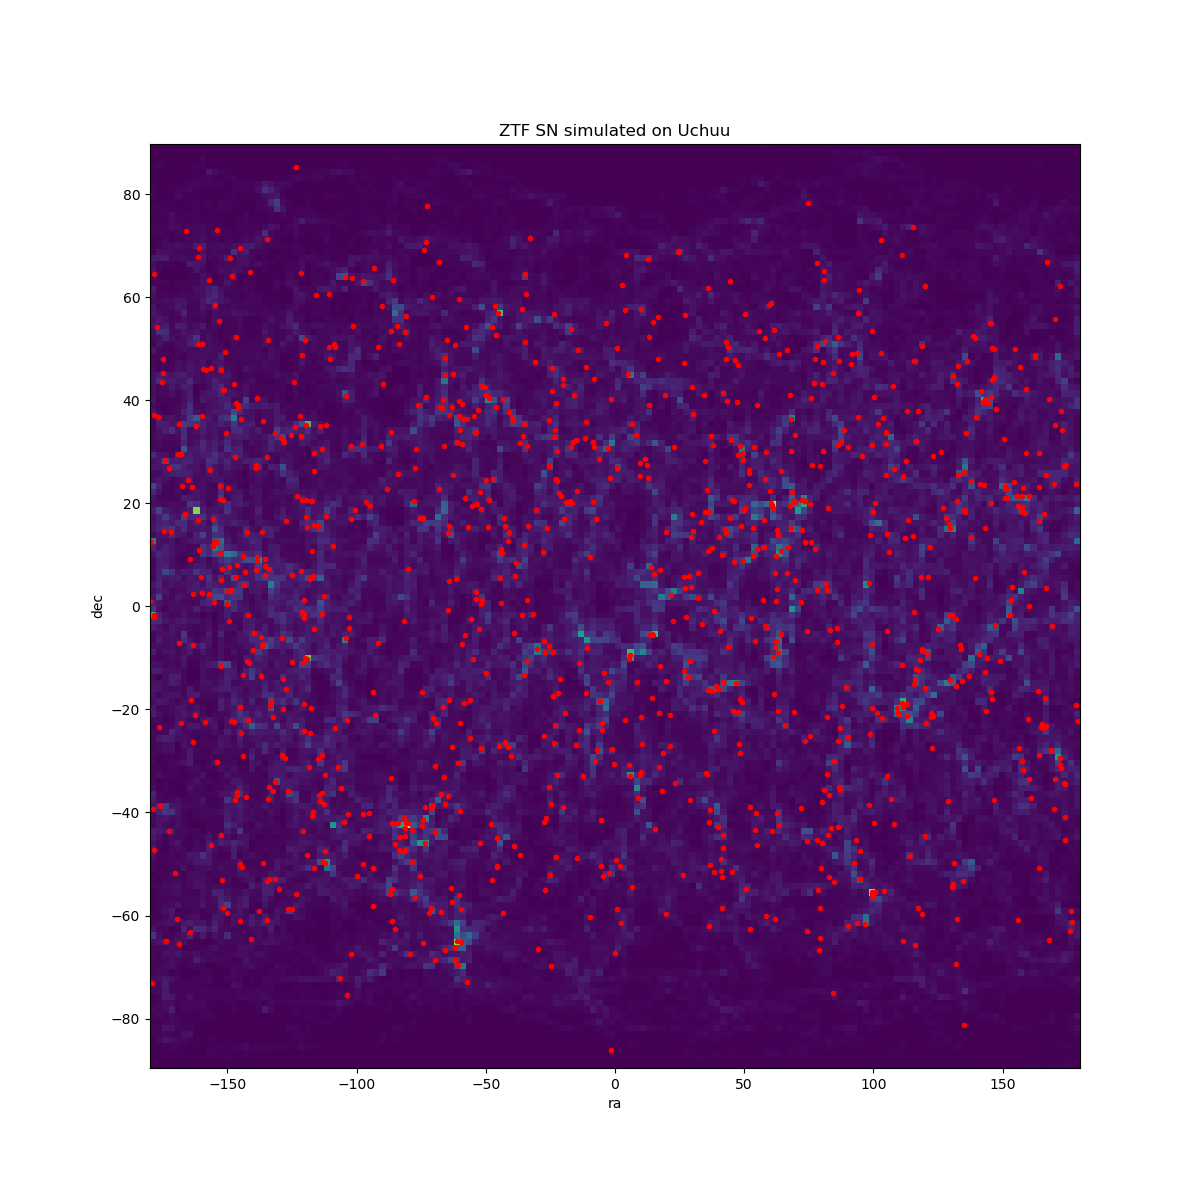
\includegraphics[width=0.9\textwidth]{MainLayout/BORG_chapter/figures/ztf_uchuu.png}
    \caption{2D full-sky projection of the Uchuu density field at redshift of $z\approx0.04$ with the ZTF supernovae simulated on top of it represented by red dots.}
    \label{fig:ztf_uchuu}
\end{figure}


\section{BORG-Peculiar Velocity}

The BORG-Peculiar Velocity (BORG-PV) algorithm is the same as the traditional BORG algorithm with the main difference being in the tracer modeling and likelihood. For BORG-PV, we 
will be using the supernovae distance moduli along with their redshifts as input. The goal will be to then infer the underlying density and velocity field as 
. One major difference with the study of galaxies is in the implementation of a bias model. 
The study of galaxy bias models has a long history with many different models having been suggested such as a linear bias (\cite{Kaiser_1984}), a nonlinear local bias (\cite{Fry_1993}) or an EFTofLSS bias (\cite{Mirbabayi_2015}) 
and there are still ongoing efforts to improve it. For the case of supernovae we will be relying on a simple phenomonological approach which will be describeed in the 
following section alongside the supernova modeling and likelihood. \\ 

\subsection{Initial likelihood}

In this section we will be describing the initial version of the BORG-PV likelihood. This likelihood was developped by Deaglan J. Bartelett during the beginning of my PhD
and it describes how well we can infer the supernova velocities. 
We denote $\mu_{\text{obs}}$ the observed distance modulus\footnote{As we explained in Chapter 2, we do not directly observe the distance modulus but instead it calculated through
the observations of supernova lightcurves. In here we assume that that $\mu_{\text{obs}}$ is the distance modulus obtained after having observed the supernova lightcurves.}, 
$z_{\text{obs}}$ the observed redshift and $\sigma_{\mu}$ is the intrinsic dispersion of supernovae. The first ingredient we need to determining the likelihood is having a prediction 
for the observed redshift. This should include the contribution of the supernova peculiar velocities with the help of the inferred velocity field. For objects at low redshift, 
Equation \ref{eqn:physical_distance} for comoving distances $r$ can be approximated as:
\begin{equation}
    r \approx \frac{c}{H_0} \left[ z - \frac{1+q_0}{2} z^2 \right]
\end{equation}
with $q_0 = \frac{\Omega_m}{2} - \Omega_{\Lambda} $. By inverting this relation for $z$, we get:
\begin{equation}
    z = \frac{1 - \sqrt{1 - 2rH_0(1+q_0)/c}}{1+q_0}
    \label{eqn:zcosmo}
\end{equation} 
For our analysis, we fix $H_0$ and $\Omega_{\Lambda}$ to a fiducial cosmology. We can then infer the cosmological redshift by knowing the distance $r$, 
given by inverting the luminosity distance relation in Equation \ref{eqn:dL_mu}, and $\Omega_m$. We 
will be denoting this redshift as $z_{\text{cosmo}}$. We can have a predicted redshift by adding the contribution of the velocity field using the following relation:
\begin{equation}
    cz_{\text{pred}}(r) = cz_{\text{cosmo}}(r) + (1+z_{\text{cosmo}}(r))v_r
\end{equation}
where $z_{\text{pred}}$ is the predicted redshift and $v_r$ is the radial projection of the velocity field at a distance $r$. We also assume that the peculiar velocities can be 
affected by sources other than the velocity field which will be modeled as a Gaussian noise $\mathcal{N}(0, \sigma_v)$.\\ 

The second ingredient would be to define a prior on the supernova distribution. If we assume a constant density of 
supernovae, than the expected number of supernova $N$ present at a distance $r$ is purely geometrical giving us:
\begin{equation}
    dN \propto 4\pi r^2 dr
\end{equation}
This means that the number of supernovae present between $r$ and $r+dr$ scales as $r^2$. Moreover, we define a supernova bias model relating the positions of supernovae with 
the evolved density field as:
\begin{equation}
    b_{SN}(r) = (1 + \delta^F(r))^{\alpha}
\end{equation}
where $\alpha$ is a free parameter. We'll call it the bias parameter. The bias parameter can exhibit four regimes:
\begin{itemize}
    \item $\alpha=0$: No bias exists and supernova do not preferential position regarding the dark matter field.
    \item $\alpha=1$: Supernova exhibits a linear bias where the number of supernova is proportional to the overdensities.
    \item $\alpha>1$: Supernova have a higher preference of being in overdense regions.
    \item $\alpha<1$: Supernova have a higher preference of being in underdense regions.
\end{itemize}
The prior on the supernova positions can then be written as:
\begin{equation}
    p_{SN}(r) = r^2 b_{SN}(r) = r^2 (1 + \delta^F(r))^{\alpha}
\end{equation}

Thirdly, we define a selection function that accounts for the fact that supernovae are not observed infinitely far away. For this, we use the following selection function:
\begin{equation}
    p_{\text{selection}}(r) = e^{-\lambda \frac{r}{R_{\text{max}}}}
\end{equation}
where $\lambda$ is a free parameter controlling the rate of decay and $R_{\text{max}}$ is the maximum comoving distance of the survey. 
This parametrisation allows for a smooth exponential decay of the expected number of supernovae with distance, avoiding the sharp 
discontinuity that would arise from a hard cutoff at $r = R_{\text{max}}$. \\

Finally, we marginalize over the distance $r$ for each supernova and normalize the likelihood, giving us:

\begin{equation}
    p(cz_{\text{obs}}|\mu_{\text{obs}})= \frac{\left( \int_{0}^{R_{\text{lim}}} dr \quad e^{- \frac{(\mu_{\text{pred}}(r) -\frac{\mu_{\text{obs}}}{\mu_A} )^2}{2\sigma_{\mu}^2} } 
    \quad e^{-\frac{(cz_{\text{pred}}(r) - cz_{\text{obs}})^2}{2 \sigma_v^2}} \quad p_{SN}(r) \quad e^{-\frac{\lambda}{R_{\text{max}}}r} \right)}{\left(\int_{0}^{R_{\text{lim}}} dr 
    \quad e^{- \frac{(\mu_{\text{pred}}(r) -\frac{\mu_{\text{obs}}}{\mu_A} )^2}{2\sigma_{\mu}^2} } 
    \quad p_{SN}(r) \quad e^{-\frac{\lambda}{R_{\text{max}}}r}\right)}
\end{equation}

Where $R_{\text{lim}}$ is the integration limit which is greater than the furthest supernova, $\mu_A$ the distance uncertainty and $\mu_{\text{pred}}(r)$ is calculated with:
\begin{equation}
    \mu_{\text{pred}}(r) = 5 \log_{10} \left( (1+z_{\text{cosmo}}(r))r \right) + 25
    \label{eqn:mu_r}
\end{equation}

\subsection{Generating self-consistent mocks}

The self-consistent supernova mocks are simulated to mach the model description above. We start by generating a random Gaussian initial density field $\delta^{IC}$ and let it evolve 
using a gravity solver until we obtain a final density field $\delta^{F}$ and a velocity field $\mathbf{v}$. We then define an amplitude function $\Phi$ containing the bias model and 
selection effects:
\begin{equation}
    \Phi(r, \phi, \theta) = (1+ \delta(r, \phi, \theta))^{\alpha}.e^{-\frac{\lambda}{R_{\text{max}}}r}
\end{equation}
The supernova are then generated by a Poisson process where a discrete generation of the cartesian coordinates from the amplitude function $\Phi$ is done. 
The number of supernovae generated is chosen beforehand. A mask is applied to ensure that the supernova generated are within the limit $R_{\text{lim}}$. We then 
calculated the observed redshift using:
\begin{equation}
    cz_{\text{obs}} = cz_{\text{cosmo}} + (1+z_{\text{cosmo}})v_r + \mathcal{N}(0, \sigma_v)
\end{equation}
where $z_{\text{cosmo}}$ is calculated using Equation \ref{eqn:zcosmo} and $v_r$ is the radial projection of the velocity field at $r$ for each supernova. The distance modulus 
is obtained the same way as Equation \ref{eqn:mu_r} and is then scattered so we get an observed distance modulus with:
\begin{equation}
    \mu_{\text{obs}} = \mu_{\text{true}} + \mathcal{N}(0, \sigma_{\mu})
\end{equation}
Finally, the right ascension and declanation angles are reported by converting the cartesian coordinates into spherical coordinates. \\

\subsection{Issues with intial likelihood}
\subsubsection{Selection function}

While testing different parameter configurations for the previously mentioned selection function, we have noticed a strong dependency in the $\lambda$ parameter that can bias the 
sampling of the other model parameters as well as the cosmology. We plot in Figure () the likelihood profile of a self-consistent simulation (see Section ref for more details on the 
simulation) for $\alpha$, the $z$-axis component of the bulkf flow $V_z$, $\Omega_m$ and $\sigma_8$ for 4 values of $\alpha$ : 1, 3, 5 and 7 while $R_{\text{max}}$ is 
fixed at $370 \text{Mpc}.h^{-1}$. 
What we notice is that all parameters are very sensitive to value of $\lambda$, more specifically that the smaller the value of $\lambda$, the more biased the parameters are. Therefore 
an incorrect initial estimation of $\lambda$ can be greatly problematic. Moreover, this choice of modeling will fail if we decide to apply our BORG-PV model on the ZTF DR2 volume 
limited sample as the selection function does not match the hard cutoff at a redshift of $z=0.06$. We can even attempt to set $\lambda$ to 0 since the volume limited sample 
should be a complete sample but this results in the same issue as seen in Figure (ref). \\

\subsubsection{Supernova prior}

Recent results from \cite{Lordet_2026} have shown that supernovae tend to be found in overly dense regions in the Universe with a large number of supernovae being present at a 
redshift of $z \approx 0.02-0.03$ creating what we see as a "bump" in the supernovae distribution accross redshift. This means that the assumption that the supernovae density is 
constant at low redshift (example of what was done in \cite{Perley_2020}) is not the most accurate description of the supernova distribution. The number of supernova 
$N_{\text{SN}}$ observed by a survey between a distance $r$ and $r+dr$ can be expressed as:
\begin{equation}
    dN = n(r) \times 4 \pi r^2 dr
\end{equation}
where $n(r)$ is the number density of supernovae. This can be related to the observed rate as:
\begin{equation}
    R(r) = \mathrm{S}(\phi, \theta, r) \frac{n(r)}{T_{\text{obs}}}
\end{equation}
where $T_{\text{obs}}$ is the time of observation and $\mathrm{S}$ is a selection function that would account for the survey's footprint, galactic extinction and any 
instrumental effects that would decrease the number of observed supernova. For our applications on self-consistent simulations and the 
ZTF-Uchuu mocks (Sections ref and ref), we will be generating supernovae on the full-sky and will not include any Malmquist bias effects. Therefore $\mathrm{S}$ becomes unity. 
If we assume a constant rate, then $dN \propto r^2 dr$ giving the $r^2$ geometric dependence in the prior described earlier. 
If we assume that this is not the case, then we get:
\begin{equation}
    dN(r) \propto n(r)r^2 dr
\end{equation}
In practice, we do not have direct access to $n(r)$ but we can infer $n(z)$. In Figure (ref) we show the $n(z)$ distribution obtained on the ZTF-Uchuu simulations obtained in 
100? bins up to a redshift of $z=0.06$. We proceed to then fit the number density with a cubic spline. The purpose of fitting with a cubic spline is to keep the $n(z)$ 
differentiable as it will be needed to then infer $n(r)$. In fact, we can relate the two number densities with:
\begin{equation}
    n(r) \propto \frac{n(z)}{4\pi r^2 \times \frac{dr}{dz}}
\end{equation}
The $\frac{dr}{dz}$ term can be deduced from Equation \ref{eqn:physical_distance} and is entirely determined by the cosmology. We get $\frac{dr}{dz} = \frac{c}{H(z)}$.
Finally, we can present a more realistic prior on supernovae expressed as:
\begin{equation}
    p_{SN}(r) \propto r^2\, n(r)\,(1+\delta^F)^{\alpha},
    \quad \text{with } n(r) \propto \frac{n(z)}{4\pi r^2 \times \frac{dr}{dz}}.
    \label{eqn:new_prior}
\end{equation}

Other motivations for this new prior lies in the ZTF-Uchuu simulations themselves. We could assume that such effects can be captured by the bias model. We 
compare self-consistent simulations with the ZTF-Uchuu simulations containing the exact same number of supernovae. We generated a set of self-consistent mocks each with 
a different value for $\alpha$. We bin the number of supernovae based on the overdensity. If the simulations are generated in the same way, we would expect to see 
a match between the bins for a given $\alpha$ value. We obtain the following Figures (ref). We notice that there isn't a singular value of $\alpha$ for which the 
self consistent simulations match the ZTF-Uchuu simulations. Moreover, we seem to notice a regime change based on the over density for the ZTF-Uchuu simulations, which 
could possibly hint that the difference can be capured using two bias model parameters. During this PhD I have not explored this avenue but instead relied on the new supernova 
prior to capture the differences between the simulations. \\



\subsection{Improved likelihood}

Our first improvement to the likelihood is in the implementation of the prior presented in Equation \ref{eqn:new_prior}. The second improvement was done by replacing the 
selection function $p_{\text{selection}}(r)$. We were inspired by the work done in \cite{Stiskalek_2025}. The method derived in the paper largely follows what was done in \cite{Kelly_2008}. Given a 
an observed dataset $\mathbf{d}_i$ for a source $i$ with source parameters $\boldsymbol{\theta}_i$ drawn from a population characterized by $\boldsymbol{\Lambda}$ 
and a selection function $S$ such that $S=1$ is the data is observed and $S=0$ if not, then the fraction of detected samples from a total population is given by:
\begin{equation}
    p(S=1|\boldsymbol{\Lambda}) = \int \int d \mathbf{d}_{\text{pred}} d \boldsymbol{\theta} p(S=1|\mathbf{d}_{\text{pred}}) \mathcal{L} 
    (\mathbf{d}_{\text{pred}}|\boldsymbol{\theta}, \boldsymbol{\Lambda})\pi (\boldsymbol{\theta}|\boldsymbol{\Lambda})
\end{equation}
where $\mathbf{d}_{\text{pred}}$ denotes the predicted data vector and $\pi$ the prior as detailed in Equation (21) of the paper. The paper to give the exact formulation when 
the selection is done on redshift, which is exactly the case for the ZTF DR2 volume limited sample. In that case, the fraction of detected samples 
is given by Equation (33) in the paper:
\begin{equation}
    p(S=1) = \int d^3 \mathbf{r} p_{SN}(\mathbf{r}) \Phi_{\text{CDF}} \left(\frac{cz_{\text{thresh}} - cz_{\text{pred}(r)}}{\sigma_v}\right)
\end{equation}
where $z_{\text{thresh}}$ is the limiting redshift ($z_{\text{thresh}}=0.06$ in our case) and $\Phi_{\text{CDF}}$ the normal cumulative distribution function. The full likelihood 
is therefore given by:
\begin{equation}
    \mathcal{L} = \prod_{i=1}^{N_\text{SN}} p(cz_{\text{obs},i}|\mu_{\text{obs},i})p(S=1)
\end{equation}
Where $i$ denotes each individual supernova. Or more simply, we can take the natural logarithm of the likelihood which gives us:
\begin{equation}
    \boxed{\log \mathcal{L} = \sum_{i=1}^{N_\text{SN}} p(cz_{\text{obs},i}|\mu_{\text{obs},i}) + N_\text{SN}p(S=1)}
\end{equation}
Where $p(cz_{\text{obs}_i}|\mu_{\text{obs}_i})$ is the likelihood of each supernova with no selection effects which is given by
\begin{equation}
    \boxed{p(cz_{\text{obs}_i}|\mu_{\text{obs}_i}) = \int_{0}^{R_{\text{lim}}} dr \quad e^{- \frac{(\mu_{\text{pred},i}(r) -\frac{\mu_{\text{obs},i}}{\mu_A} )^2}{2\sigma_{\mu}^2} } 
    \quad e^{-\frac{(cz_{\text{pred},i}(r) - cz_{\text{obs},i})^2}{2 \sigma_v^2}} \quad r^2\, n(r)\,(1+\delta^F(r))^{\alpha}}
\end{equation}